\chapter{Zarządzanie budżetem oraz predykcja wydatków przy użyciu znanych metod analizy danych}
\section{Wprowadzenie}
Z zagadnieniem zarządzania budżetem domowym spotyka się każdy, kto dysponuje środkami pieniężnymi. Oznacza ono analizę wszystkich poniesionych kosztów oraz planowanie przyszłych wydatków. Prawidłowe zarządzanie budżetem pozwala na świadome i przemyślane wydawanie pieniędzy oraz ułatwia oszczędzanie.

Na zarządzanie budżetem istnieje wiele sposobów. Najprostszym i najstarszym z nich jest prowadzenie dziennika dochodów i wydatków. Usprawnieniem tego procesu są liczne aplikacje ułatwiające prowadzenie budżetu domowego przez wykorzystanie komputera lub smartfona. Udostępniają one szereg funkcjonalności, które sprawiają, że rejestracja przychodów i wydatków staje się łatwiejsza. Samo rejestrowanie kosztów nie pozwala jednak na ich planowanie, przez co zarówno tradycyjne podejście do zarządzania budżetem, jak i istniejące aplikacje do tego służące nie są w pełni funkcjonalne.
 
Powstała aplikacja na podstawie danych o przychodach i rozchodach wszystkich użytkowników pozwala na \textbf{predykcję}, czyli przewidywanie wydatków powiązanych z zakupem produktów lub usług, które niosą za sobą koszty utrzymania, np. samochodu.
\section{Dostępne aplikacje do zarządzania budżetem}
Na rynku jest dostępnych wiele aplikacji służących do zarządzania budżetem, zarówno płatnych, jak i darmowych. Poddane analizie zostały trzy aplikacje wykorzystywane w tym celu: \textbf{Kontomierz, YNAB} i \textbf{Spendee}.

\textbf{Kontomierz} (rys. \ref{kontomierz_interfejs}) jest darmową aplikacją dostępną poprzez przeglądarkę internetową oraz aplikacje na systemy Android oraz iOS. Pobiera ona dane o wydatkach użytkownika z historii transakcji na koncie bankowym. Aplikacja ta prezentuje użytkownikowi w przejrzysty sposób strukturę wydatków wraz z ich kategoriami, propozycje oszczędności oraz usług bankowych. Jest zintegrowana z systemami wielu polskich banków, dzięki czemu w szybki sposób umożliwia orientację w bieżącej sytuacji finansowej użytkownika. Jest to najpopularniejsza aplikacja do zarządzania budżetem na polskim rynku.
\begin{figure}[!ht]
	\begin{center}
		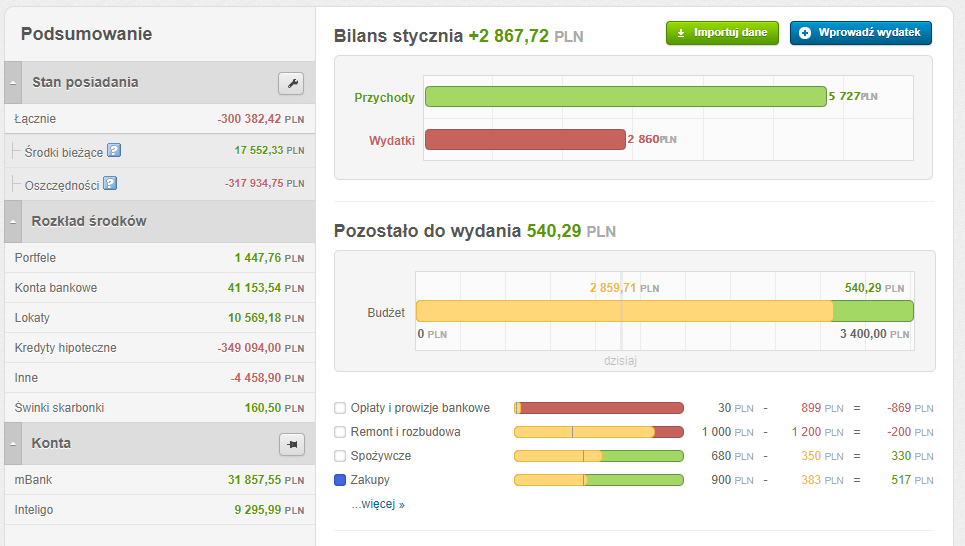
\includegraphics[width=6in]{img/aplikacje/kontomierz_interfejs.png}
		\caption{Interfejs aplikacji Kontomierz}
		\label{kontomierz_interfejs}
	\end{center}
\end{figure}

\textbf{YNAB - You Need A Budget} (rys. \ref{ynab_interfejs}) to aplikacja dostępna w języku angielskim, zarówno poprzez przeglądarkę internetową, jak i przez aplikacje mobilne, służąca do kompleksowej rejestracji i planowania budżetu. Podobnie jak Kontomierz, posiada możliwość importu danych z konta bankowego, jednak z racji tego, iż nie jest to polska aplikacja, nie ma możliwości importu danych z polskich banków.\\
YNAB jest jedną z bardziej rozbudowanych aplikacji dostępnych na rynku, aczkolwiek nie jest aplikacją darmową,  dostępny jest jedynie miesięczny bezpłatny okres próbny. W skład jej funkcjonalności wchodzi automatyczna rejestracja wydatków i przychodów oraz kompleksowy system planowania budżetu. Wszystkie wolne środki jakie posiadamy przypisujemy do wybranych celów, którymi są planowane wydatki, opłaty stałe bądź oszczędności.
\begin{figure}[!ht]
	\begin{center}
		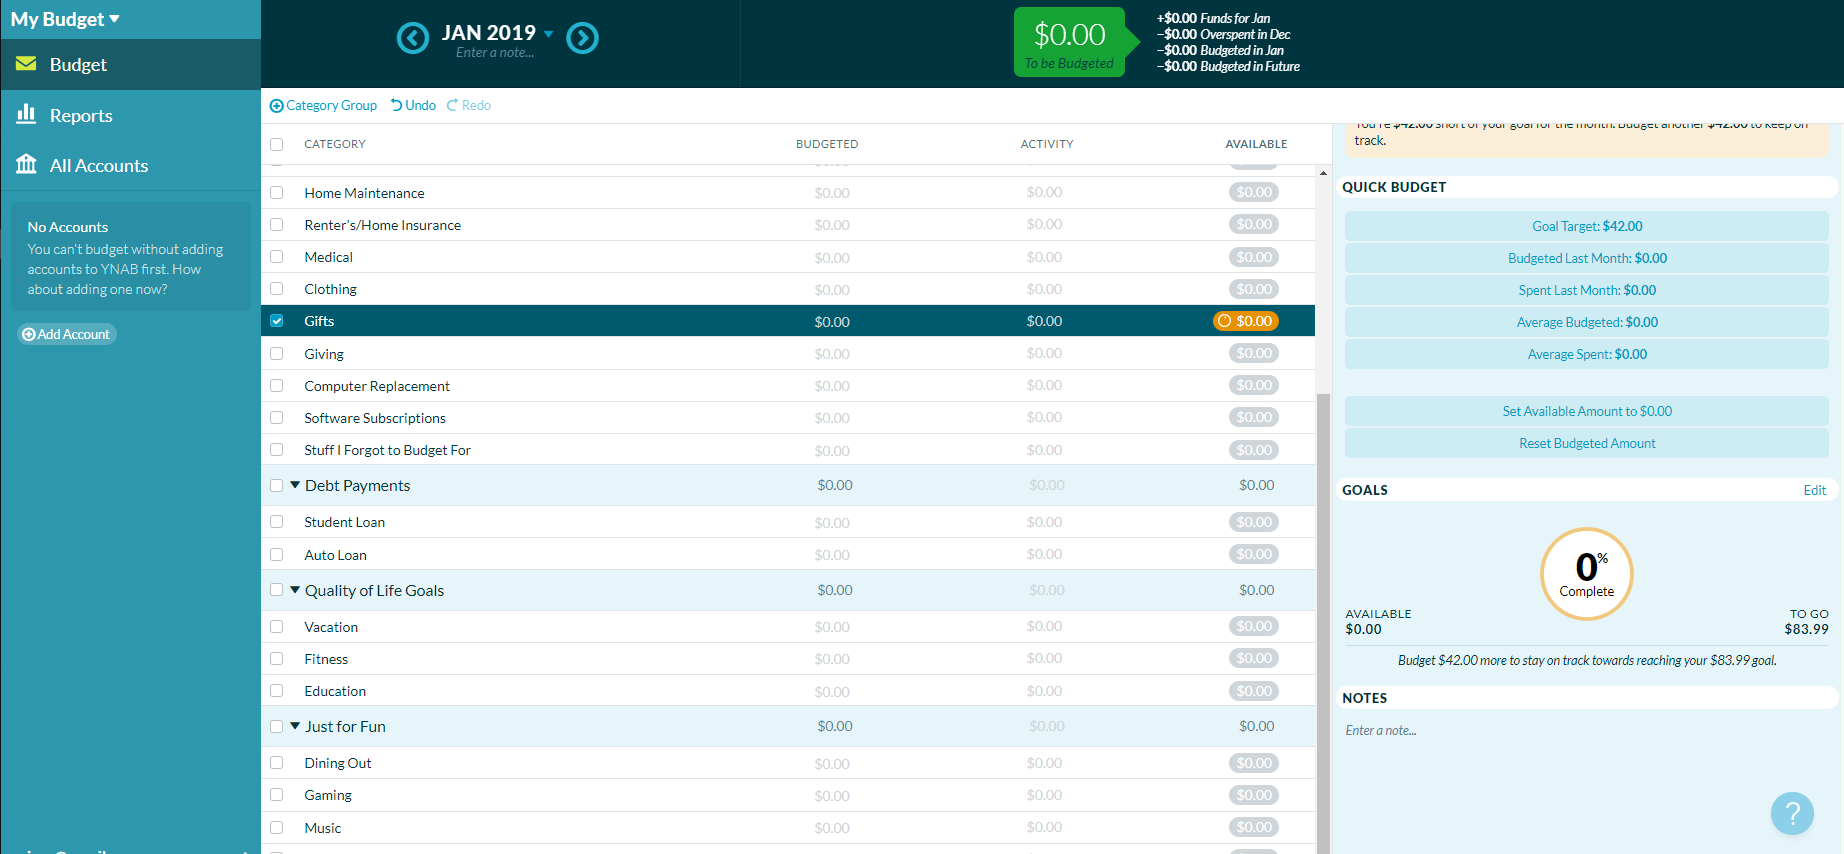
\includegraphics[width=6in]{img/aplikacje/ynab_interfejs.png}
		\caption{Interfejs aplikacji YNAB}
		\label{ynab_interfejs}
	\end{center}
\end{figure}

\textbf{Spendee} (rys. \ref{spendee_interfejs}) jest aplikacją anglojęzyczną służącą do zarządzania budżetem. Jest dostępna zarówno w formie aplikacji webowej, jak i mobilnej. Aplikacja posiada wersję podstawową oraz dwie wersje płatne różniące się dostępnymi funkcjonalnościami. Pakiet podstawowy jest darmowy oraz oferuje możliwość wprowadzania i przeglądu wydatków oraz dochodów użytkownika.\\
Wersje płatne oferują znacznie więcej funkcjonalności. Aplikacja pozwala na automatyczny import danych z systemów bankowych oraz, w przeciwieństwie do YNAB, obsługuje banki z wielu krajów, w tym także z Polski. Wykupując wersję premium użytkownik dostaje również możliwość dzielenia wirtualnego portfela z innymi użytkownikami oraz automatyczną kategoryzację wydatków przy imporcie danych z systemu bankowego.
\begin{figure}[!ht]
	\begin{center}
		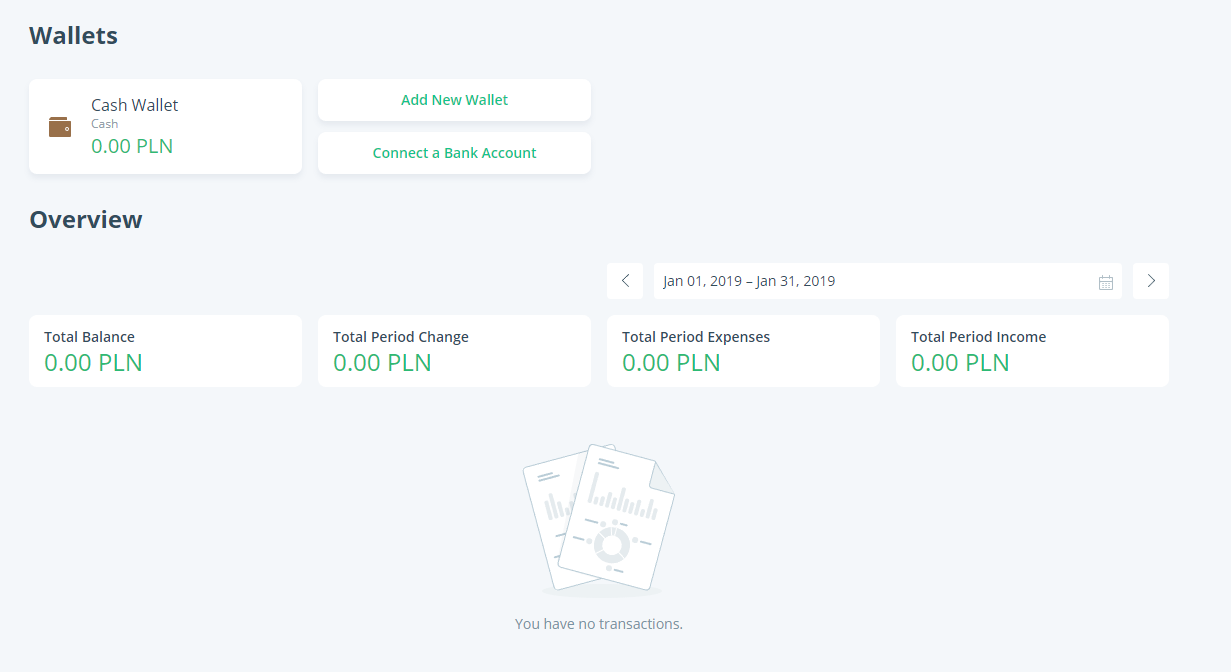
\includegraphics[width=6in]{img/aplikacje/spendee_interfejs.png}
		\caption{Interfejs aplikacji Spendee}
		\label{spendee_interfejs}
	\end{center}
\end{figure}

\section{Objaśnienie pojęć z dziedziny komputerowej analizy danych finansowych}
\textbf{Statystyka} to nauka o metodach badań poświęconych liczbowo wyrażalnym właściwościom zbiorowości oraz wszelkie prace związane z gromadzeniem i opracowaniem masowych danych liczbowych.\cite{bptstatystyka}

\textbf{Analiza regresji} jest statystyczną metodologią przewidywania wartości jednej lub więcej zmiennych odpowiedzi (zależnych) za pomocą zbioru predyktorów (czyli zmiennych niezależnych). Może być także użyta do oszacowania efektów jakie predyktory wywierają na odpowiedzi.\cite{wielowymiarowymodelregresjiliniowej2014}

\textbf{Predykcja (prognozowanie)} to przewidywanie jakie wartości przyjmie zmienna objaśniana przy zadanej wielkości zmiennej objaśniającej.\cite{bptstatystyka}
\section{Opis wybranych metod analizy danych}\label{metody_analizy_danych}
\subsection{Wieloraka regresja liniowa} \label{regresja}
Niech \(z_1, z_2, ..., z_k\) będą zbiorem \(k\) predyktorów, które potencjalnie wpływają na zmienną \(Y\). Model regresji liniowej \(n\)-elementowej próbki:
\[Y_n = \beta_0 + \beta_1z_{n1} + \beta_2z_{n2} + \dots + \beta_kz_{nk} + \epsilon_n\]
gdzie \(\beta_i, i = 0, 1, ..., k\) są nieznanymi i ustalonymi współczynnikami regresji,\\
\(\beta_0\) jest wyrazem wolnym,\\
\(\epsilon\) jest błędem losowym.\cite{wielowymiarowymodelregresjiliniowej2014}

Dla zbioru \(n\) rekordów danych model regresji możemy zapisać w postaci macierzowej: \[Y = X\beta + \epsilon\]
gdzie\\
\(Y = \begin{bmatrix}
y_1 \\
y_2 \\
\vdots \\
y_n
\end{bmatrix}\) - macierz zmiennych zależnych,\\
\(X = \begin{bmatrix}
1 & x_{11} & x_{12} & \dots & x_{1k} \\
1 & x_{21} & x_{22} & \dots & x_{2k} \\
\vdots & \vdots & \vdots & & \vdots \\
1 & x_{n1} & x_{n2} & \dots & x_{nk} \\
\end{bmatrix}\) - macierz predyktorów,\\
\(\beta = \begin{bmatrix}
\beta_0 \\
\beta_1 \\
\vdots \\
\beta_n
\end{bmatrix}\) - macierz współczynników regresji,\\
\(\epsilon = \begin{bmatrix}
\epsilon_1 \\
\epsilon_2 \\
\vdots \\
\epsilon_n
\end{bmatrix} \) - macierz reszt. \cite{martinabremer2012}
\subsection{Regresja nieparametryczna}
\textbf{Regresja nieparametryczna}, w odróżnieniu od regresji parametrycznej (np. \ref{regresja}), nie uwzględnia ścisłego matematycznego modelu regresji, ale próbuje oszacować postać zależności między predyktorami \(X\) oraz zmienną zależną \(Y\). Dzięki tej cesze regresja nieparametryczna znajduje zastosowanie w przypadkach, w których postać zależności między predyktorami a zmienną zależną nie jest ściśle określona.\cite{nonparametricregression}
Przykładem regresji nieparametrycznej jest metoda \textbf{k najmniejszych kwadratów}. Polega ona na przybliżeniu wartości zmiennej zależnej jako średniej wartości \(k\) najbliższych rekordów znanych danych.
\[f(x)=\sum_{i = 1}^{n}w_i(x)y_i \]
gdzie:\\
\(n\) - liczba próbek,\\[10pt]
\(w_i(x) = \left\{\begin{array}{ll}
1/k\;je\dot{z}eli\;x_i\;jest\;jednym\;z\;k\;najbli\dot{z}szych\;do\;x\;rekord\dot{o}w,\\
0\;w\;przeciwnym\;wypadku,
\end{array}
\right. \)\\[10pt]
\(y_i\) - wartość \(i\)-tej zmiennej zależnej.\cite{ryantibshirani}

\textbf{Odległość rekordów} definiuje się za pomocą metryk, np. metryki euklidesowej. Określa się ją jako:
\[d(x,y)=\sqrt{\sum_{i=1}^{n}(x_i-y_i)^2} \],
gdzie:\\
\(x, y\) - dwa zbiory danych,
\(x_i, y_i\) - \(i\)-ta cecha zbioru \(x\) lub \(y\).\cite{rachelski}
\subsection{Metoda najmniejszych kwadratów}\label{najmniejsze_kwadraty}
\textbf{Metoda najmniejszych kwadratów} jest metodą wyznaczenia współczynników regresji parametrycznej polegającą na znalezieniu takich ich wartości, aby zminimalizować rozrzut między wartościami rzeczywistymi i odpowiadającymi im wartościami teoretycznymi zmiennej, czyli zminimalizować sumę kwadratów reszt.\cite{bptstatystyka}

W najlepszym wypadku różnica między wartościami rzeczywistymi i teoretycznymi wynosi 0, zatem reszta \(\epsilon\) dla każdego rekordu danych jest równa 0. W takim wypadku model regresji można zapisać następująco: 
\[Y = X\beta\]
Przekształcając powyższe równanie otrzymujemy:
\[Y - X\beta = 0\]
\[X^T(Y - X\beta) = 0 \]
\[X^TY - X^TX\beta = 0 \]
\[X^TX\beta = X^TY\]

Stąd macierz współczynników regresji wyznaczamy w następujący sposób:
\[\beta = (X^TX)^{-1}X^TY\]
gdzie\\
\(X\) - macierz predyktorów,\\
\(Y\) - macierz zmiennych zależnych.\cite{martinabremer2012}\\
Przedstawione operacje na macierzach \(X^T\) i \(X^{-1}\) to odpowiednio \textit{transpozycja macierzy} oraz \textit{odwrócenie macierzy}.
\iffalse
\textbf{Transpozycją macierzy \(A\)} nazywamy macierz \(A^T\) której wierszami są kolumny macierzy transponowanej \(A\).
\fi
\section{Wykorzystanie metod analizy danych do predykcji wydatków}
Predykcja wydatków w stworzonej aplikacji wiąże się z tzw. \textbf{wydatkami głównymi}. Są to wydatki, które generują dodatkowe, występujące przez kilka następnych miesięcy, koszta. Użytkownik, po wprowadzeniu kategorii oraz wielkości wydatku głównego, na podstawie danych o wydatkach wszystkich użytkowników, dostaje predykcję kosztów związanych ze wspomnianym wydatkiem w miesiącach po nim następujących.

W niniejszej pracy użyta została parametryczna regresja wieloraka (\ref{regresja}) wraz z metodą najmniejszych kwadratów (\ref{najmniejsze_kwadraty}). Metody te zostały wybrane, gdyż zbiór danych, na których dokonujemy predykcji jest ściśle ustrukturyzowany oraz możliwe jest określenie matematycznego modelu opisującego zależności w nim występujące.

Model regresji skonstruowany na potrzeby predykcji posiada trzy predyktory: miesięczny dochód użytkownika, wielkość wydatku dla którego wykonywana jest predykcja oraz suma wydatków z prognozowanej kategorii. Współczynniki regresji wyznaczane są przy pomocy metody najmniejszych kwadratów opisanej w rozdziale \ref{najmniejsze_kwadraty}. Dla prognozy na każdy kolejny miesiąc tworzony jest model regresji, koszta w każdym miesiącu obliczane są przy użyciu innych współczynników regresji.

Dostępne na rynku aplikacje do zarządzania budżetem zapewniają kompleksowe rozwiązania służące do rejestracji wydatków i dochodów oraz planowania budżetu. Ich funkcjonalność może być wzbogacona o aspekt prognozowania wydatków. Mógłby on być szczególnie przydatny przy planowaniu przyszłych kosztów oraz ich integracji z istniejącym budżetem.